\documentclass[reprint, nofootinbib]{revtex4-2} %preprint: 1
\usepackage[utf8]{inputenc}
\usepackage{graphicx}
\usepackage{float}
% math symbols
\usepackage{amsmath}
\usepackage{xcolor}
\usepackage{amssymb}
\usepackage{amsfonts}

% pic
\usepackage{graphicx}
\usepackage{dcolumn}
\usepackage{bm}
\usepackage{hyperref}
\usepackage{mathptmx}
\newcommand{\ud}{\,\mathrm{d}}

\begin{document}
\title{PS3203 Computational Physics: Midterm 2020}
\author{Hyejin Kim (20185055)}
%\affiliation{GIST college, Gwangju 61005, Republic of Korea}
\email[email: ]{aadeliee@gm.gist.ac.kr}
\date{\today}

\maketitle
\section{Problem 1}
The motion of damped harmonic oscillator is described with differential equation,
\begin{equation}\label{eqn:DHO}
	\ddot{x}+2\gamma\dot{x}+\omega_0^2x = 0
\end{equation}
where $\gamma$ is the damping factor, and $\omega_0$ is the natural frequency with no damping factor. The general solution for equation~\eqref{eqn:DHO} is~\cite{CMbook}
\begin{equation}\label{eqn:DHOsol}
	x(t) = e^{-\gamma t}\left(A_1e^{\sqrt{\gamma^2-\omega_0^2}t}
	+A_2e^{-\sqrt{\gamma^2-\omega_0^2}t}\right)
\end{equation}
There are four cases classified with the magnitude of $\gamma$. When $\gamma=0$, it is called no damping case, and the solution is simply the well-known harmonic oscillator.
\begin{equation}
	x(t) = A\cos(\omega_0t-\delta)
\end{equation}
For $\gamma^2<\omega_0^2$ case, it is called underdamping, which also shows oscillatory motion with
\begin{equation}
	x(t) = Ae^{-\gamma t}\cos\left(\sqrt{\omega_0^2-\gamma^2}t-\delta\right)
\end{equation}
Moreover $\gamma^2=\omega_0^2$, the degenerated case. In other words, critical damping. This case of system doesn't show oscillation anymore.
\begin{equation}
	x(t) = (A+Bt)e^{-\gamma t}
\end{equation}
Lastly, for case $\gamma^2>\omega_0^2$, this is called overdamping, and we use equation~\eqref{eqn:DHOsol} directly.

From the calculated solutions, consider a phase space consist of $(x, \dot{x})$. This phase diagram is plotted in Figure~\ref{fig:fig1} by integrating equation~\eqref{eqn:DHO} with small time step $\ud t=0.01$ each. Also I only considered positive damping factor.

For the first case (a), as there is no damping factor, it has the phase diagram of simple harmonic oscillator having no loss of energy. We can also observe the maximum velocity is $A\omega_0 = A/2$, making the trajectory oval. Here, amplitude is in range $0.25\leq A \leq 1$.

The underdamped motion (b) shows similar oscillatory motion with previous case, but with energy loss. For weak damping $\gamma=0.05$, it shows clear spiral trajectory. For strong damping $\gamma=0.25$, it spirals into origin faster than weak-damping case. Here, initial starting point from $x, \dot{x}$-intersection with oval $x^2+2\dot{x}^2=1$, total 4 points.

The critical damped motion (c), the system does not goes into oscillatory motion. The trajectories also seem to have single asymptotic path along $\dot{x} = -\gamma x$. In this case, the system experiemces fastest approach to equilibrium into origin. Here, initial starting point from each point on oval $x^2+2\dot{x}^2=1$, total 16 points.

The last case, the overdamped case (d), almost all trajectories goes along line $\dot{x} = -(\gamma-\omega_2)x$ and approaches equilibrium, where $\omega_2 = \sqrt{\gamma^2-\omega_0^2}$. It is important that most system starts moving simmilar to asmptotic path $\dot{x} = -(\gamma+\omega_2)x$. Here, initial starting point same as case (c).

\begin{figure}[t]
	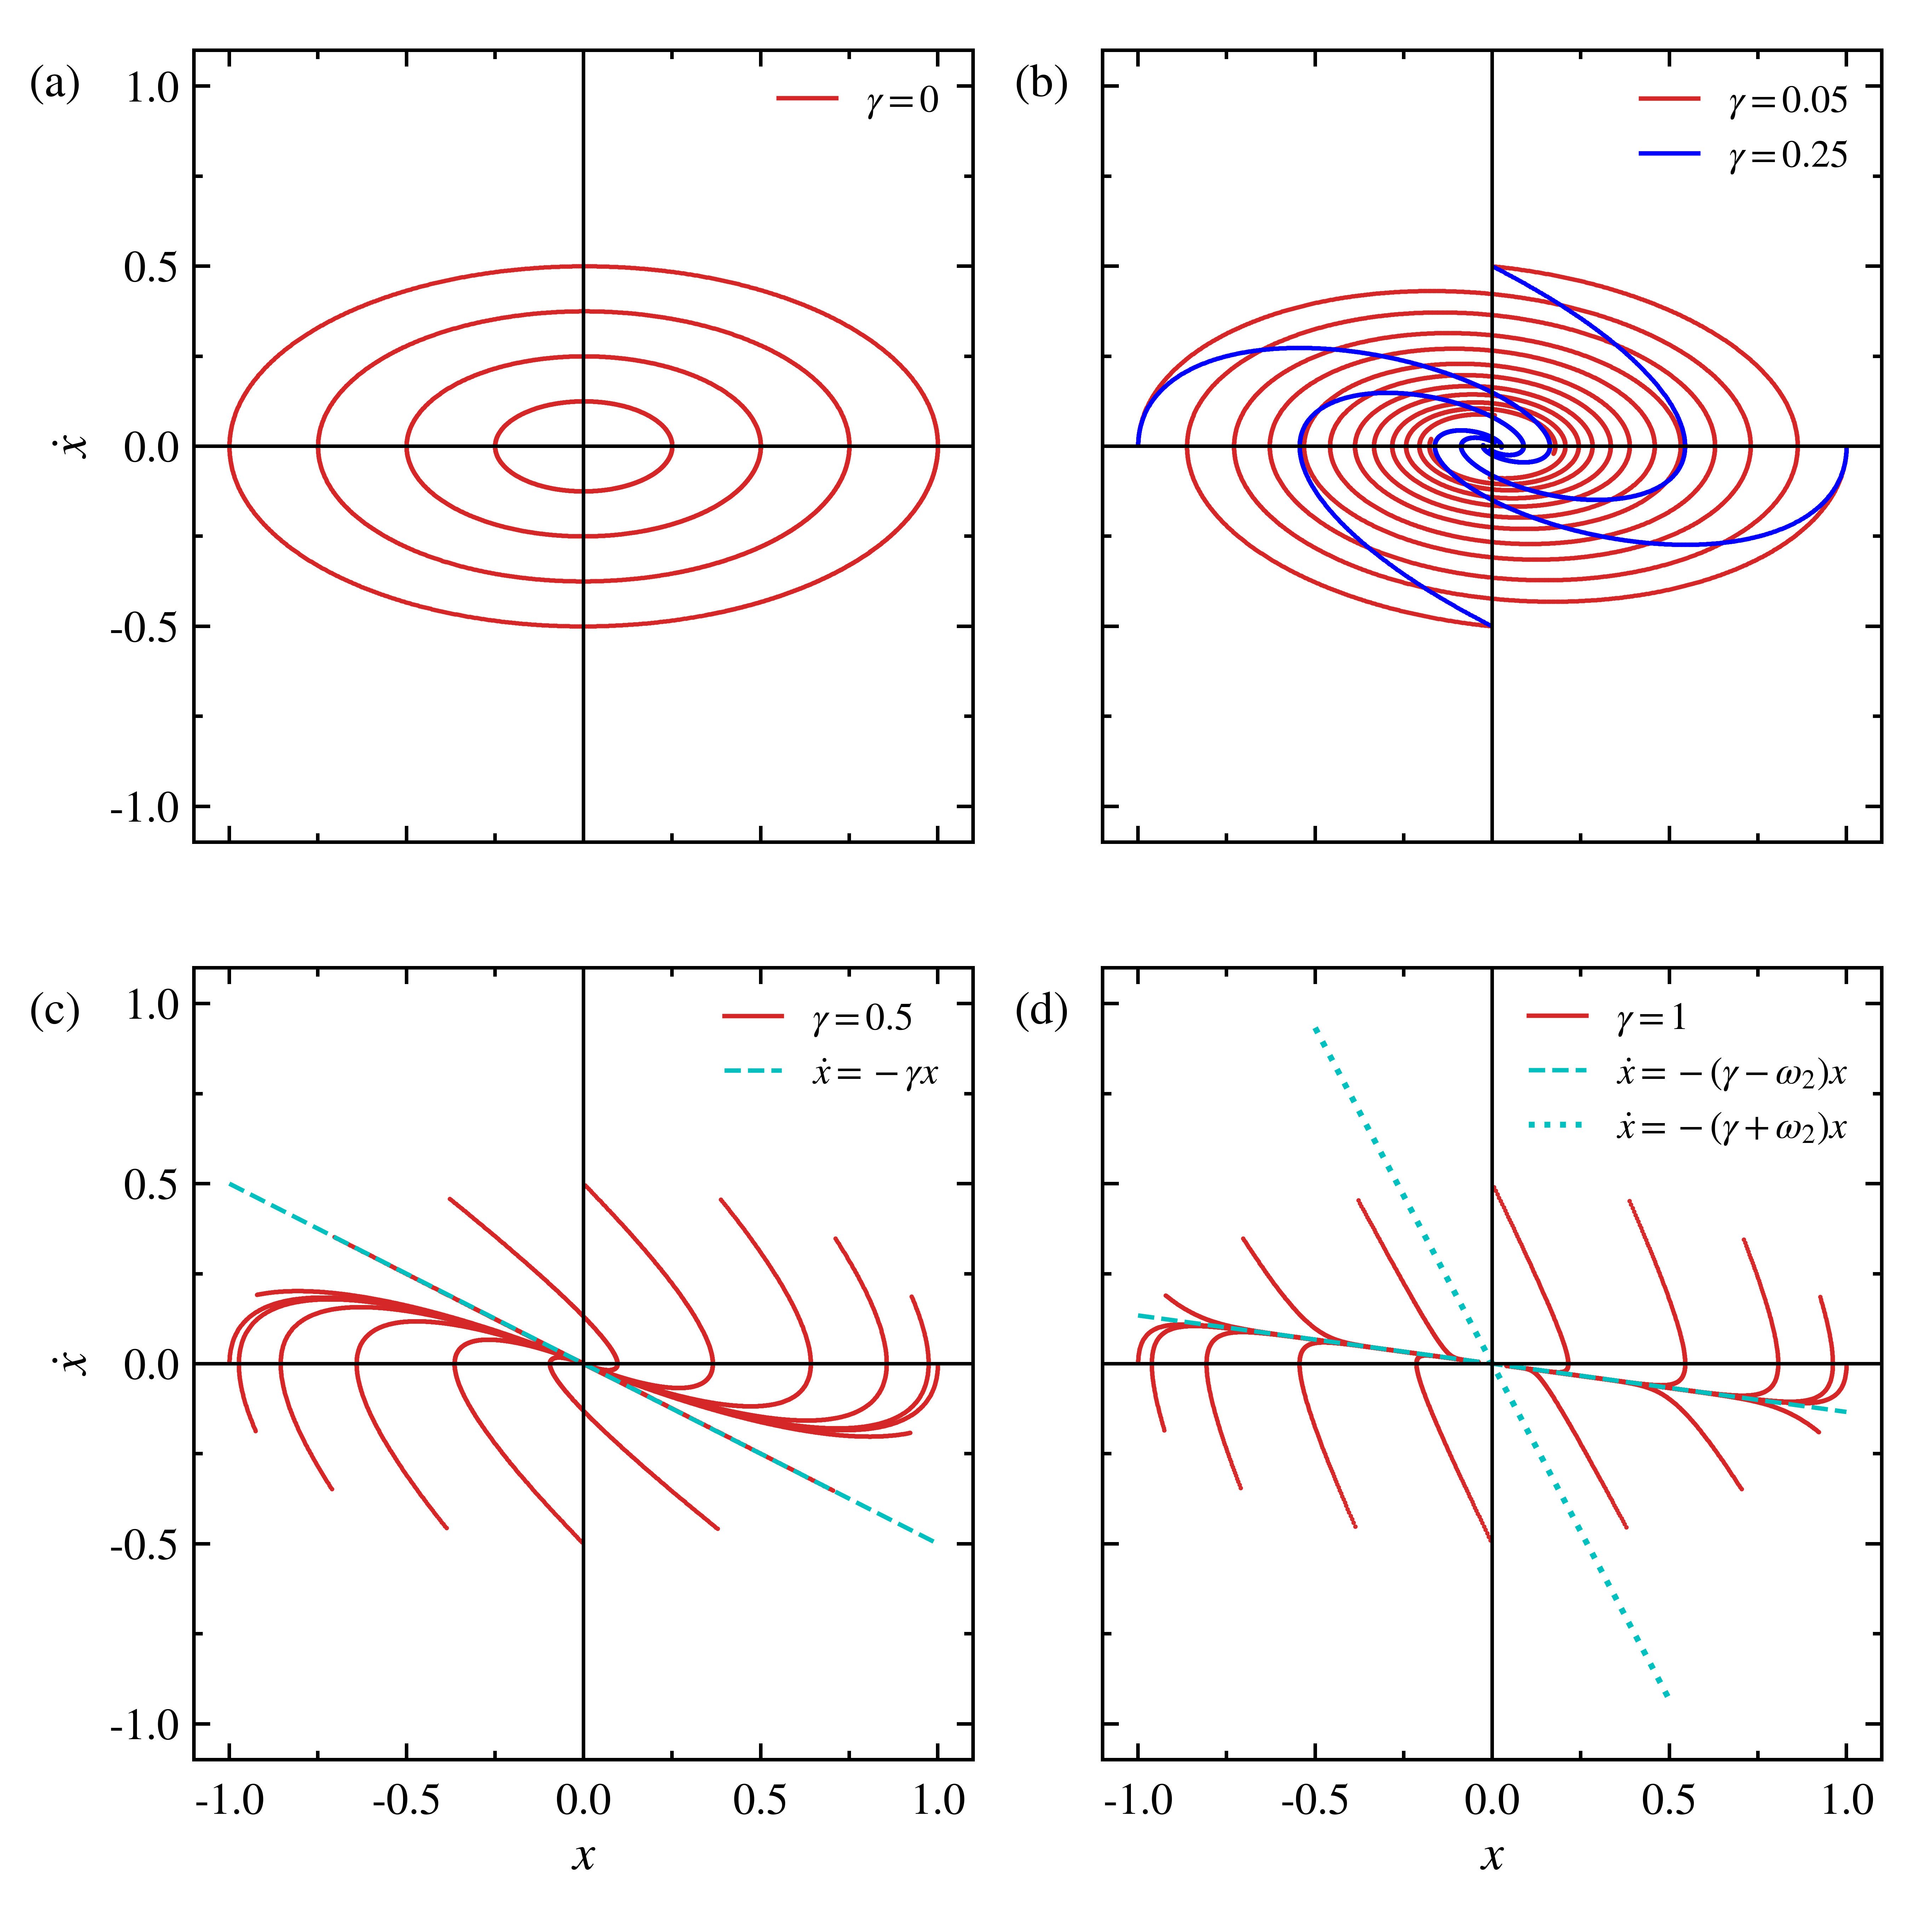
\includegraphics[width=0.48\textwidth]{fig1_add.png}
	\caption{Phase diagram $(x, \dot{x})$ of 4 different cases: (a) No damping (b) Underdamping (c) Critical damping, (d) Overdamping}
	\label{fig:fig1}
\end{figure}

\section{Problem 2}
We are interested in the non-linear recurrence relation which is given by
\begin{equation}\label{eqn:relation}
	x_{n+1} = a x_n(1-x_n^2), \quad a = 2.5
\end{equation}
The stability of solution $\lim_{n\to\infty}x_n$ has strong correlation with parameter $a$. Brief explanation related to this stability problem is on section~\ref{sec:appA}. 

Here, we will concentrate on initial value problem. Starting from two slightly different initial values $x_0 = 0.9000000$ and $0.9000001$, I will find $n$ where two different calculation diverge more than 30\%. This rate were calculated using below equation.
\begin{equation}
	r = \left\vert\frac{x_n(x_0=0.9000000)-x_n(x_0=0.90000001)}{(x_n(x_0=0.9000000)+x_n(x_0=0.90000001))/2}\right\vert
\end{equation} 
This two calculation was performed using different precision, 32-float and 64-float. The overall calculation is illustrated on Figure~\ref{fig:fig2}.

Surprisingly, for two different precision, starting point of diverge were same as $n=29$. It is strange that 6 and 15 significant digits (each using float32 and 64) makes no difference on initial value problem. However, there are still difference between different precision, in Figure~\ref{fig:fig3}. 

\begin{figure}[t]
	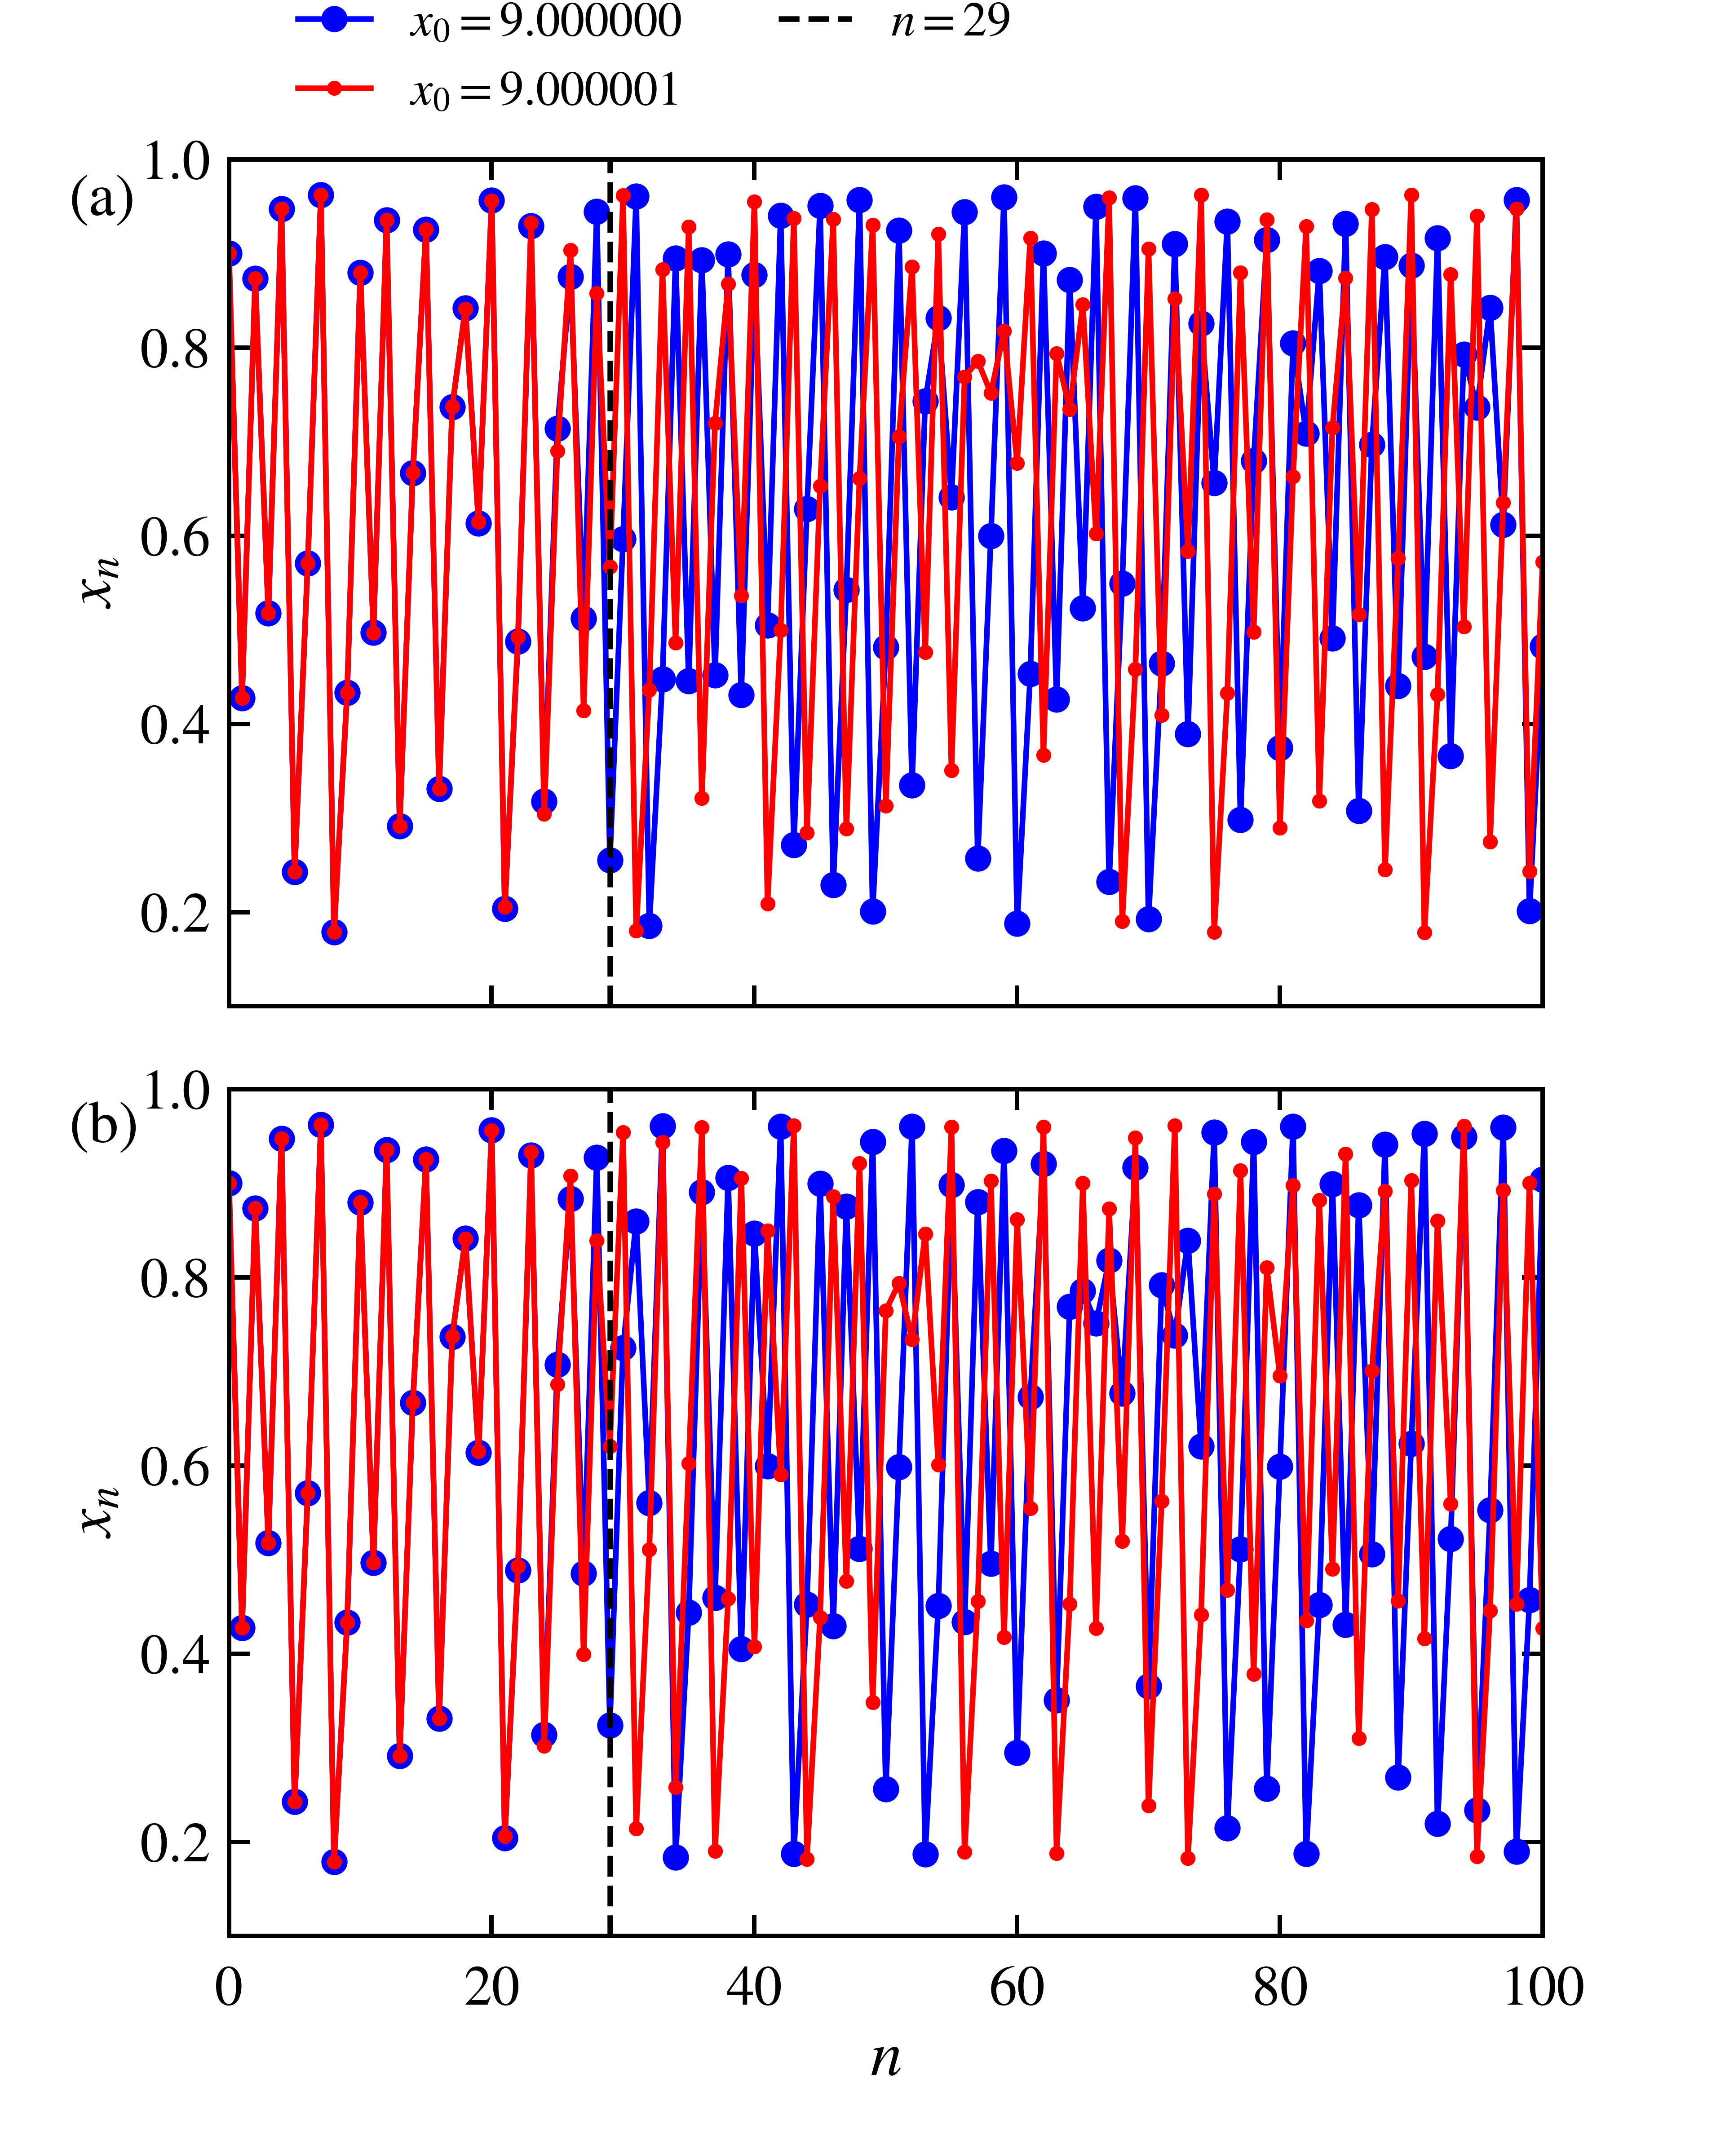
\includegraphics[width=0.45\textwidth]{fig2.png}
	\caption{$x_n$ calculation with 100 iteration: Performed with (a) 32-bit float precision (b) 64-bit precision.}
	\label{fig:fig2}
\end{figure}

Figure~\ref{fig:fig3} indicates the same calculation as Figure~\ref{fig:fig2} with larger iteration. In this figure, we can see clear pattern after large iteration in plot (a) and (b), which uses float32. 

Compared to ploat (c) and (d) with 64-bit precision, 32-bit precision shows discrete structure on $x_n$ solution, which means more cutoff of digits due to precision issue. This indicates that using 32-bit float causes some data loss after large iteration, and becomes less accurate in calculation.\\ 

\appendix
\begin{figure}[H]
	\includegraphics[width=0.48\textwidth]{fig3.png}
	\caption{$x_n$ calculation with $10^4$ iteration: (a) $x_0=0.9000000$ with float32 (b) $x_0=0.9000001$ with float32 (c) $x_0=0.9000000$ with float64 (d) $x_0=0.9000001$ with float64. }
	\label{fig:fig3}
\end{figure}
\section{Bifurcation diagram}\label{sec:appA}
Using bifurcation diagram, we can determine the stable solutions of given relation~\cite{Bdiagram}. From Figure~\ref{fig:bifurcation}, what we can confirm is that at $a=2.5$, one can observe unstable solution on range approximately 0.2 to 1.0, for positive starting point. Below diagram were plotted using 64-bit float.

\begin{figure}[b]
	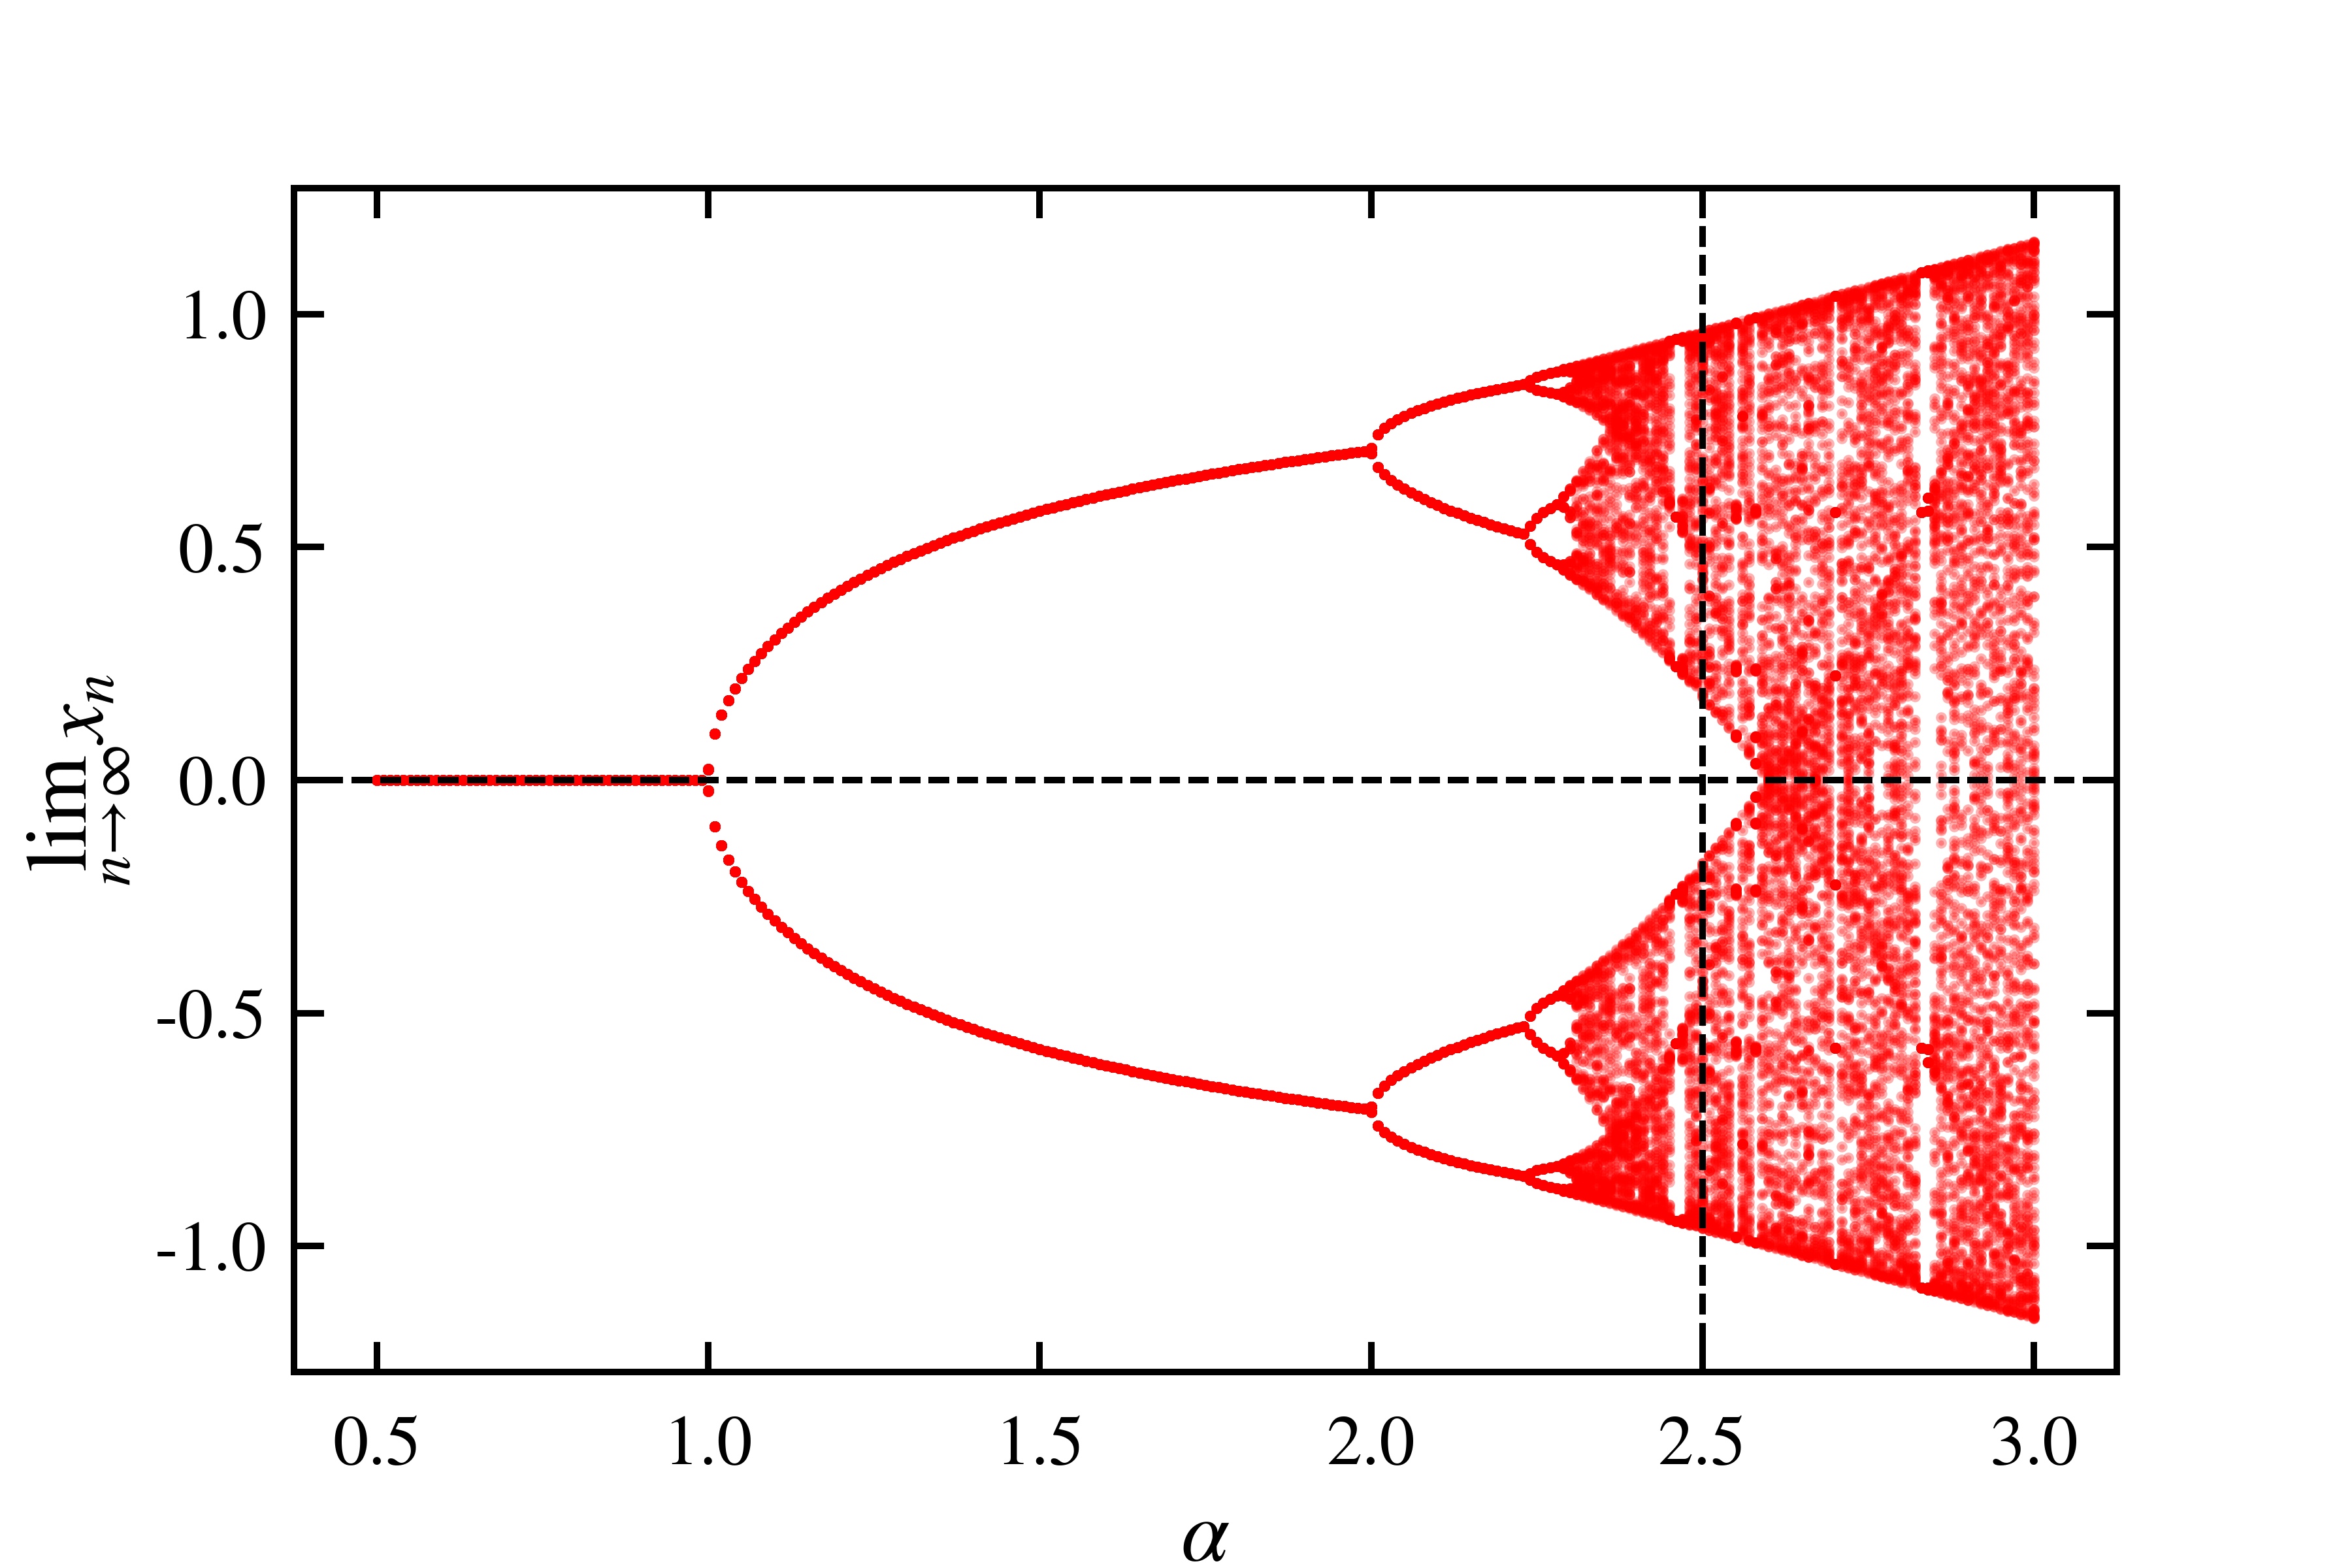
\includegraphics[width=0.43\textwidth]{bifurcation.png}
	\caption{Bifurcation diagram of equation~\eqref{eqn:relation}.}
	\label{fig:bifurcation}
\end{figure}

%\section{Problem 2 with 16-bit float}
%\begin{figure}[h] 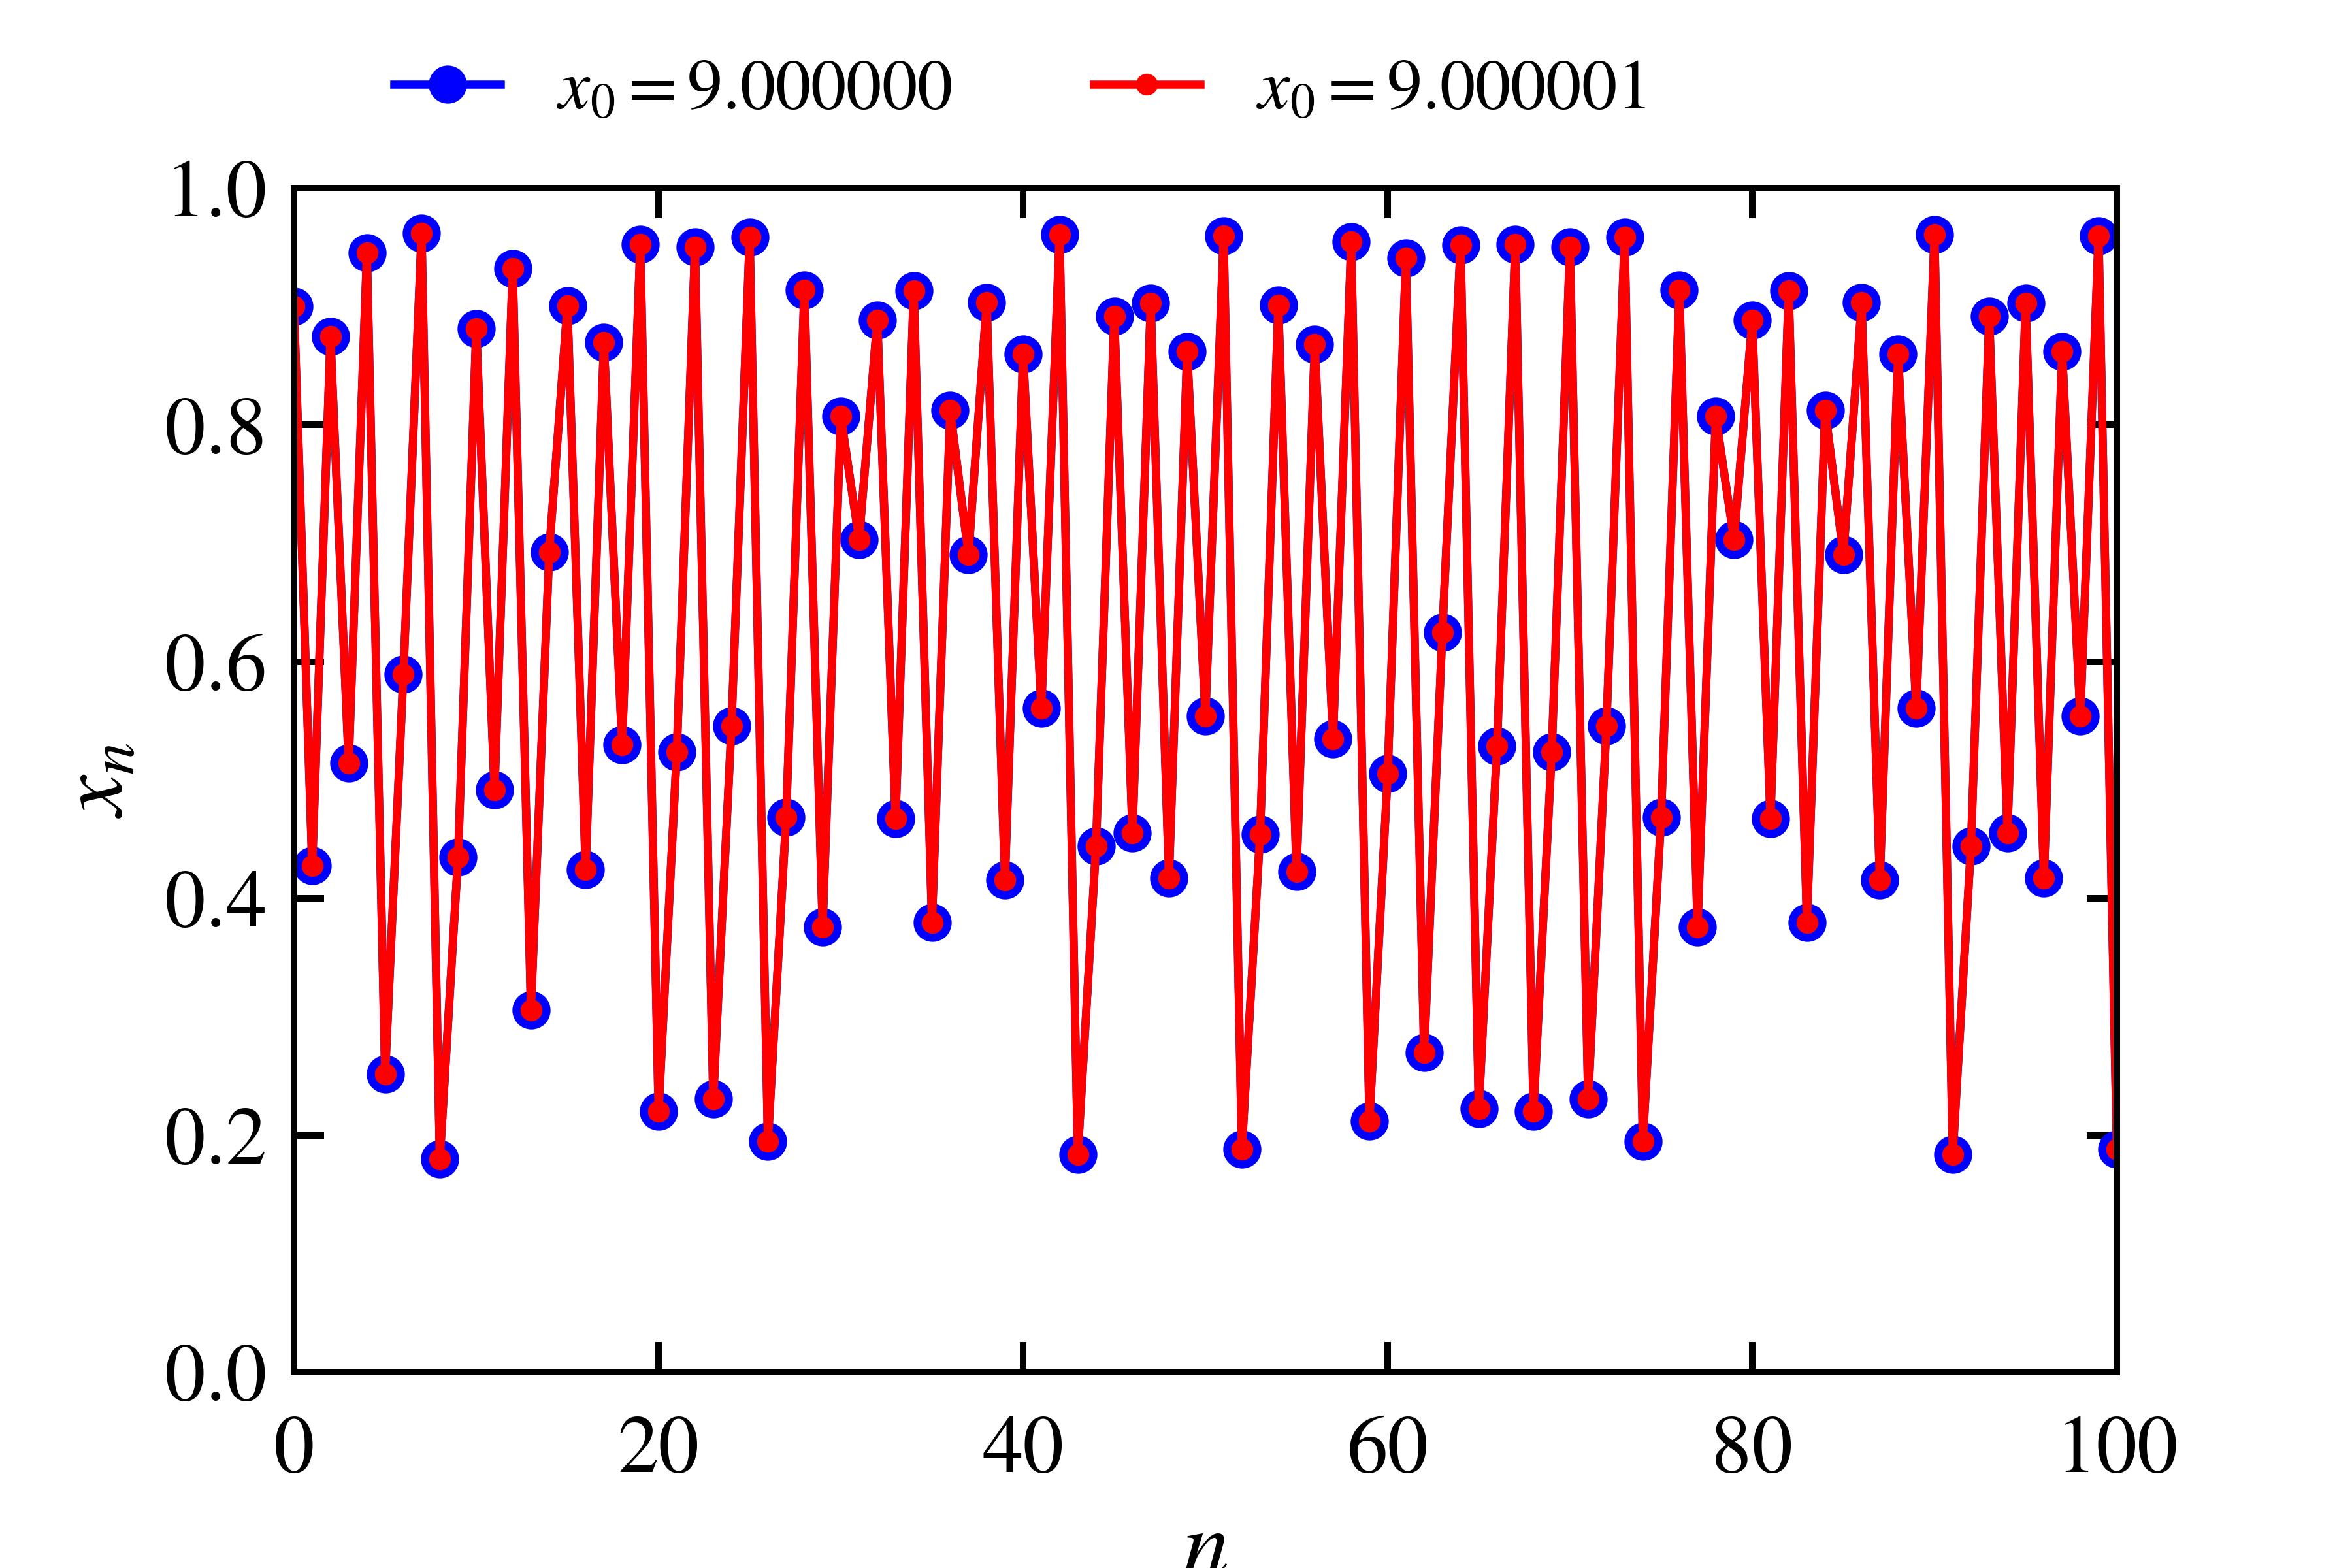
\includegraphics[width=0.45\textwidth]{fig2_add.png} \caption{Performing problem 2 using 16-bit float precision.} \label{fig:fig2add} \end{figure}



\bibliography{mid_ref}
\end{document}
